% Version 2024
%

\chapter*{Datos de la Asignatura}
\label{chap:00.datos.de.IyA}
  \addcontentsline{toc}{chapter}{Datos de la Asignatura}

  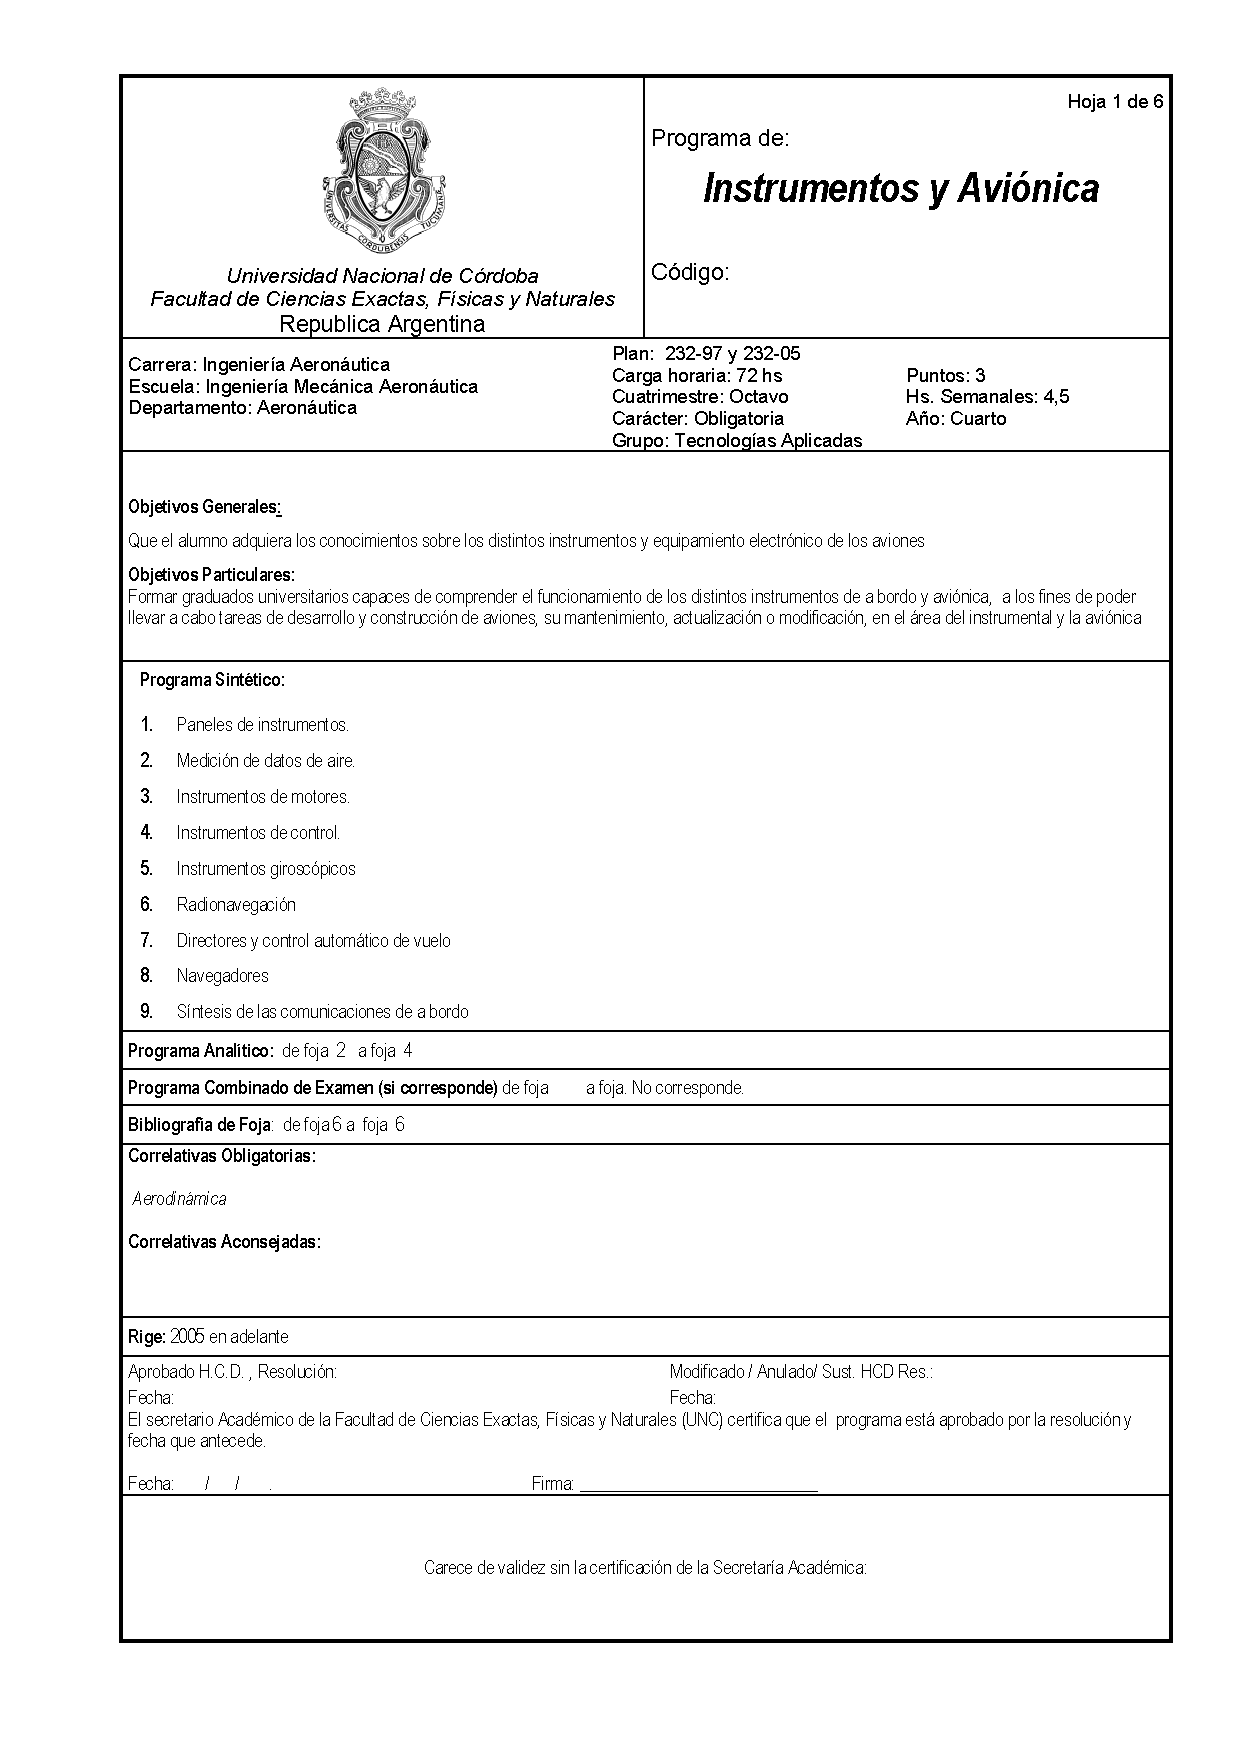
\includepdf[pages=-, fitpaper=false, scale=0.90, %landscape=true,
  offset = 0 -20,
  pagecommand={\thispagestyle{fancy}}]
  {00.Datos.IyA/Instrumentos_Y_Avionica.pdf}


\section{Días y horarios de clases}
\label{sec:dias+horarios.clases}

La asignatura se dicta de manera sincrónica/presencial en el año 2024
los días jueves de 15:45 hs a 20:15 hs.

Para las clases sincrónicas se emplea Google Meet,
 el link a la clase de la asignatura es: \\
\href{https://meet.google.com/vpm-vdau-qrq}{https://meet.google.com/vpm-vdau-qrq}
 % \url{https://classroom.google.com/c/MzY3MDEyNzQ1MjA2?cjc=wbdwdwc}

Para las clases presenciales y las evalauaciones se empleará el aula asignada a tal efecto.

El material de estudio y comunicaciones con la Cátedra se realiza a través de Google Meet cuyo link es: \\
\href{https://classroom.google.com/c/Njk3NTIwODU1Mzk4}{https://classroom.google.com/c/Njk3NTIwODU1Mzk4}



\section*{Adecuación transitoria de la metodología de cursada  y evaluación \mbox{segundo} semestre 2024}
\label{00.Adecuacion.transitoria}
  \addcontentsline{toc}{section}{Adecuación transitoria de la metodología de cursada   y evaluación  segundo semestre 2024}


\subsection*{Modalidad de enseñanza} 

Las clases se dictarán algunas de forma SINCRÓNICA y otras con PRESENCIALIDAD FÍSICA entre los docentes y los alumnos.

El día de dictado de clases será el jueves de cada semana de 15:45 a 20:

Material de estudio, asignación de tareas mediante Google Classroom


\subsection*{Modalidad de evaluación}

Las evaluaciones serán con presencialidad física de los alumnos/as.

Cantidad de parciales dos (2).

Las/los estudiantes que hayan desaprobado un (1) examen parcial teórico/práctico, si el restante examen parcial fue aprobado, tienen derecho a un (1) recuperatorio, cuya nota reemplazará a la del examen parcial reprobado.

Coloquio  tomados con presencialidad física de los alumnos/as. Cantidad uno (1).

\subsection*{Condiciones Transitorias de Regularidad}

\begin{itemize}
\item Estar correctamente matriculado para el cursado de la asignatura
\item Aprobar con nota no inferior a 4 (cuatro) cada uno de los  dos (2) exámenes parciales. 

\item Presentar y aprobar los trabajos prácticos
\end{itemize}

\subsection*{Condiciones Transitorias de Aprobación definitiva (Promoción) }


\begin{itemize}
\item Haber aprobado las correlativas previas o aprobar las que se encuentren pendientes dentro del plazo de validez de la regularidad.

\item  Estar correctamente matriculado para el cursado de la
  asignatura.
\item Aprobar con nota no inferior a 4 (cuatro) cada uno de los dos (2) exámenes parciales. 
\item Aprobar un coloquio integrador con nota no inferior a 4 (cuatro)
\item Presentar y aprobar los trabajos prácticos
\end{itemize}



\section*{Cronograma para el dictado de la Asignatura a\~no 2024}
\label{sec:00.cronograma}
  \addcontentsline{toc}{section}{Cronograma para el dictado a\~no 2024}

  \begin{itemize}
  \item Capítulo 1. Paneles de Instrumentos (GARCIA) 8/08/2024
  \item Capítulo 6. Radionavegación (OLIVA) 15/08/2024
  \item Capítulo 6. Radionavegación (GARCIA) 22/08/2024    
  \item Capítulo 9. Síntesis de las comunicaciones de a bordo (OLIVA)     29/08/2024
  \item \textbf{Parcial 01,  05/9/2024 Abarca Capítulos 1, 6, 9.  PRESENCIAL}

  \item Capítulo 8. Navegadores (SORIA) 12/9/2024 {\bf CLASE PRESENCIAL}
  \item Capítulo 8. Navegadores (GPS, nav. inerc.) (GIRAUDO) 19/9/2024    
    
  \item Capítulo 7. Directores y control automático de vuelo ( SORIA) 26/09/2024  {\bf CLASE PRESENCIAL}
  
    \item Capítulo 4. Instrumentos de control. 
          Capítulo 3. Instrumentos de motores (GIRAUDO) 03/10/2024
  
  \item Capítulo 2. Medición de datos de aire (GALEASSO) 10/10/2024
  \item Capítulo 5. Instrumentos giroscópicos (GALEASSO) 17/10/2024   {\bf CLASE PRESENCIAL}

  \item {\bf Parcial 02,  24/10/2024 Abarca Capítulos 2, 3, 4 , 5 , 7 y 8. PRESENCIAL}

  \item \textbf{Recuperatorios Parciales.  31/10/2024. PRESENCIAL}

    
  \item {\bf Clase de consulta. Entrega de TPs. 07/11/2024 }

  \item \textbf{Coloquio,  14/11/2024 Abarca todo el programa. PRESENCIAL}
  \item \textbf{Coloquio, 21/11/2024 Abarca todo el programa. PRESENCIAL}
  \end{itemize}


\section*{Docentes}
\label{00.docentes}
\addcontentsline{toc}{section}{Docentes}

{\small
  \begin{tabular}{llm{0.40\textwidth}} \rowcolor{yellow!30}
 {\bf Docente} & {\bf Correo electr\'onico} & {\bf D\'ia, horario consulta, medio de consulta} \\ \rowcolor{cyan!20}
  Ing. Jorge GARCIA & jgarcia@unc.edu.ar & {  Mi\'ercoles, de 15 a 17 hs, correo electr\'onico, google meet }\\ 
  Ing. Angel  GALEASSO & angel.galeasso@unc.edu.ar & D\'ia Mi\'ercoles, de 16 a 17 hs, correo electr\'onico, google meet    \\ \rowcolor{cyan!20} 
    Ing. Pedro GIRAUDO  & pedrogiraudo@unc.edu.ar &  D\'ia Mi\'ercoles, de 17:30 a 19 hs, correo electr\'onico, google meet, zoom     \\

    Ing. Luis Mario SORIA CASTRO & luis.soriacastro@unc.edu.ar &
    \\ \rowcolor{cyan!20}
    Msc. Ing. Facundo OLIVA CUNEO & facundo.olivacuneo@unc.edu.ar & \\ \hline
  \end{tabular}
  }